\documentclass[tikz,border=12pt]{standalone}
\usepackage[T1]{fontenc}
\usepackage{mathpazo}
\usepackage{amsmath,amssymb}
\usetikzlibrary{arrows.meta, positioning, calc, fit, decorations.pathreplacing}

\definecolor{stblue}{HTML}{7B97AD}
\definecolor{rwgold}{HTML}{B8995E}
\definecolor{sage}{HTML}{7A9A7E}
\definecolor{dkbrown}{HTML}{3D3530}
\definecolor{wmgray}{HTML}{7B7067}
\definecolor{cream}{HTML}{F9F6F0}
\definecolor{border}{HTML}{D4C9B8}
\definecolor{terracotta}{HTML}{C47A6A}
\definecolor{lavender}{HTML}{907EA0}

\begin{document}
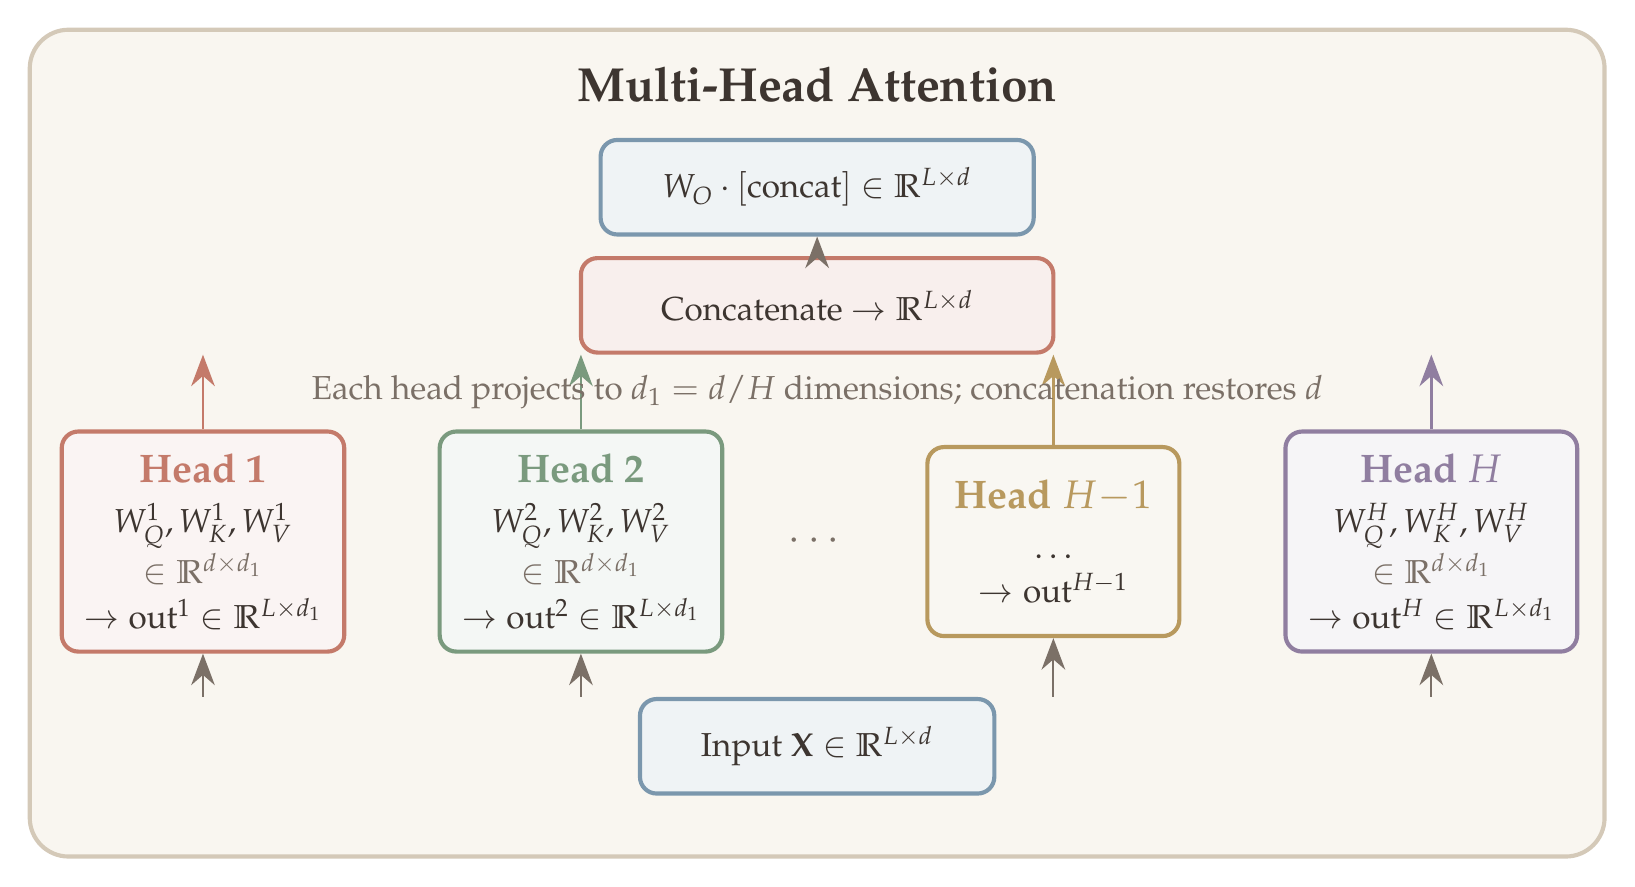
\begin{tikzpicture}[
  >={Stealth[length=4mm, width=3mm]},
  every node/.style={text=dkbrown, font=\large},
  headbox/.style={rounded corners=6pt, line width=1.5pt, minimum height=2.4cm, minimum width=3.2cm, align=center, inner sep=8pt},
]

% Background
\fill[cream, rounded corners=14pt] (0,0) rectangle (20,10.5);
\draw[border, line width=1.5pt, rounded corners=14pt] (0,0) rectangle (20,10.5);

% Title
\node[font=\LARGE\bfseries, text=dkbrown] at (10,9.8) {Multi-Head Attention};

% Output projection (top)
\node[headbox, fill=stblue!12, draw=stblue, minimum width=5.5cm, minimum height=1.2cm] (output) at (10,8.5) {$W_O \cdot [\mathrm{concat}] \in \mathbb{R}^{L \times d}$};

% Concatenate box
\node[headbox, fill=terracotta!12, draw=terracotta, minimum width=6.0cm, minimum height=1.2cm] (concat) at (10,7.0) {Concatenate $\to \mathbb{R}^{L \times d}$};

% Arrow from concat to output
\draw[wmgray, line width=1.2pt, ->] (concat.north) -- (output.south);

% Head 1
\node[headbox, fill=terracotta!8, draw=terracotta] (h1) at (2.2,4.0) {%
  {\Large\bfseries\color{terracotta}Head 1}\\[4pt]
  $W_Q^1, W_K^1, W_V^1$\\[1pt]
  {\color{wmgray} $\in \mathbb{R}^{d \times d_1}$}\\[2pt]
  $\to \mathrm{out}^1 \in \mathbb{R}^{L \times d_1}$
};

% Head 2
\node[headbox, fill=sage!8, draw=sage] (h2) at (7.0,4.0) {%
  {\Large\bfseries\color{sage}Head 2}\\[4pt]
  $W_Q^2, W_K^2, W_V^2$\\[1pt]
  {\color{wmgray} $\in \mathbb{R}^{d \times d_1}$}\\[2pt]
  $\to \mathrm{out}^2 \in \mathbb{R}^{L \times d_1}$
};

% Dots
\node[font=\Large, text=wmgray] at (10,4.0) {$\cdots$};

% Head H-1
\node[headbox, fill=rwgold!8, draw=rwgold] (h3) at (13.0,4.0) {%
  {\Large\bfseries\color{rwgold}Head $H\!-\!1$}\\[4pt]
  $\ldots$\\[2pt]
  $\to \mathrm{out}^{H-1}$
};

% Head H
\node[headbox, fill=lavender!8, draw=lavender] (h4) at (17.8,4.0) {%
  {\Large\bfseries\color{lavender}Head $H$}\\[4pt]
  $W_Q^H, W_K^H, W_V^H$\\[1pt]
  {\color{wmgray} $\in \mathbb{R}^{d \times d_1}$}\\[2pt]
  $\to \mathrm{out}^H \in \mathbb{R}^{L \times d_1}$
};

% Arrows from heads to concat
\draw[terracotta, line width=1pt, ->] (h1.north) -- (concat.south -| h1.north);
\draw[sage, line width=1pt, ->] (h2.north) -- (concat.south -| h2.north);
\draw[rwgold, line width=1pt, ->] (h3.north) -- (concat.south -| h3.north);
\draw[lavender, line width=1pt, ->] (h4.north) -- (concat.south -| h4.north);

% Input box (bottom)
\node[headbox, fill=stblue!12, draw=stblue, minimum width=4.5cm, minimum height=1.2cm] (inp) at (10,1.4) {Input $\mathbf{X} \in \mathbb{R}^{L \times d}$};

% Arrows from input to each head
\draw[wmgray, line width=0.8pt, ->] (inp.north -| h1.south) -- (h1.south);
\draw[wmgray, line width=0.8pt, ->] (inp.north -| h2.south) -- (h2.south);
\draw[wmgray, line width=0.8pt, ->] (inp.north -| h3.south) -- (h3.south);
\draw[wmgray, line width=0.8pt, ->] (inp.north -| h4.south) -- (h4.south);

% Dimension annotation
\node[font=\large, text=wmgray] at (10,5.9) {Each head projects to $d_1 = d/H$ dimensions; concatenation restores $d$};

\end{tikzpicture}
\end{document}
